\documentclass{article}
\usepackage{graphicx}
\usepackage[a4paper, bottom=1.75cm, top=1.75cm, footskip=0.85cm, left=2.5cm, right=2.5cm]{geometry}
\usepackage{indentfirst}
\usepackage{titlesec}
\titlespacing*{\section}{0pt}{2mm}{2mm}
\titlespacing*{\subsection}{0pt}{1.75mm}{1.75mm}
\titlespacing*{\subsubsection}{0pt}{1.5mm}{1.5mm}
\usepackage[hidelinks]{hyperref}
\usepackage{enumerate}
\usepackage{listings}
\usepackage{amsmath}
\usepackage{adjustbox}
\usepackage{subfig}
\setcounter{page}{0}
\graphicspath{ {./images/} }
\newcommand{\fakesection}[1]{%
	\par\refstepcounter{section}% Increase section counter
	\sectionmark{#1}% Add section mark (header)
	\addcontentsline{toc}{section}{\protect\numberline{\thesection}#1}% Add section to ToC
	% Add more content here, if needed.
}

\begin{document}
\begin{titlepage}
	
	\newcommand{\HRule}{\rule{\linewidth}{0.5mm}} % Defines a new command for the horizontal lines, change thickness here
	
	\centering % Center everything on the page
	
	%----------------------------------------------------------------------------------------
	%	HEADING SECTIONS
	%----------------------------------------------------------------------------------------
	
	\textsc{\LARGE Aalto University}\\[1.5cm] % Name of your university/college
	
\includegraphics[scale=0.5]{aaltologo.png}\\[1cm] % Include a department/university logo - this will require the graphicx package
	\textsc{\Large Data Science Project}\\[0.5cm] % Major heading such as course name
	\textsc{\large CS-C3250}\\[0.5cm] % Minor heading such as course title
	
	%----------------------------------------------------------------------------------------
	%	TITLE SECTION
	%------------------------------------------------------------5----------------------------
	
	\HRule \\[0.4cm]
	{ \huge \bfseries Interactive Biodiversity Infographics}\\[0.4cm] % Title of your document
	\HRule \\[1.5cm]
	
	%----------------------------------------------------------------------------------------
	%	AUTHOR SECTION
	%----------------------------------------------------------------------------------------
	
	\begin{minipage}{0.7\textwidth}
		\centering
		 \large
			\emph{Authors:}\\
			Aaron \\
			Behram \\
			Chau \\
			Hung \\
			Ilya \\
			Kerkko \\
			Linh \\
			Nghi \\
		
		
	\end{minipage}\\[2cm]
	
	% If you don't want a supervisor, uncomment the two lines below and remove the section above
	%\Large \emph{Author:}\\
	%John \textsc{Smith}\\[3cm] % Your name
	
	%----------------------------------------------------------------------------------------
	%	DATE SECTION
	%----------------------------------------------------------------------------------------
	
	{\large \today}\\[2cm] % Date, change the \today to a set date if you want to be precise
	
	\vfill % Fill the rest of the page with whitespace
	
\end{titlepage}

\tableofcontents

\newpage

\setcounter{section}{-1}
\fakesection{Abstract}

\begin{abstract}
Science education has benefited greatly from advances in technology: the availability and accessibility of information has increased, and pedagogical methods evolved. Teachers are able to demonstrate the impact of taught topics more efficiently and students apply new information in imaginative ways. A possible application of enhancing science education with technology comes from visualizations, which can help support students to conceptualize newly learned phenomena.
\par
This report describes the process of students from Aalto University in creating interactive infographics for visualizing biodiversity in Finland. The result of the project was a website with interactive maps and graphs as well as related information supporting students in learning about biodiversity and the relationships between species. We will cover the project assignment, the data used for modeling biodiversity and species habitats, our process of problem-solving throughout the project, as well as the mathematical and programmatic methods implemented in the solution we ended up with. Finally, the finished product will be described and its use cases demonstrated. In addition, we will share conclusions from the project and lessons learned from working as a team of data consultants. The project was associated with the Data Science Project course at Aalto University and conducted in collaboration with Reaktor.
\par
\centering
\url{https://biodiversity.streamlit.app/}
\end{abstract}

\section{About the project}
The project was assigned by representatives of Reaktor as an exercise in working as a team of data consultants for a client. In the exercise, the client was the author of a biology textbook, looking to acquire interactive web info pages about biodiversity to support their materials. We were instructed to take lead on the implementation of the website, while assuring the product follows the client’s goals. A dataset of species observations form laji.fi was to be used to model and visualize biodiversity, as well as build and publish an implementation of the web page. Associations to possible underlying factors affecting biodiversity were also to be explored.

\section{Data}
The dataset used is an extensive collection of species observations from laji.fi, consisting of approximately 49 million datapoints. The dataset is collected by private individuals from all over Finland: they have reported observations of nearly 47 thousand species, spanning over decades [1]. In our final website implementation, 13 million of these observations were used.
\par
While crowd-sourced datasets are cheap to collect and available to everyone, such data can include strong bias – in the case of the laji.fi dataset, this applied both locationally and temporally. We found the observations to be unevenly distributed around large population centers like cities and towns, as well as other locations in which observations are often made such as national parks and popular vacation destinations. Similarly, the datapoints were commonly dated from June to August, which is likely when observers have had most time for their close-to-nature hobby of logging species observations.
\par
These causes of bias led to problems with data sparsity and increased the difficulty of reliable analysis of biodiversity in Finland. When modeling biodiversity, the relative abundance of species as well as the number of differing species is of high interest: the bias made it essentially impossible to directly tell from the data whether a low number of observations in an area was due to low biodiversity, or simply caused by a lack of people to log observations. Later sections of this report describe methods we used to mitigate the effects of bias on our analysis.
\section{Methods}
To explore the raw data and present it in a nice, understandable way, we used different methods and approaches. Every approach aims to expose different sides of the data and biodiversity in Finland. While some of the approaches are based on the statistical reality of the raw data, some of them are based on the factual knowledge gathered from different sources.
\subsection{Biodiversity metrics}
To measure the biodiversity of a given community, there are several metrics serving that purpose. In our webpage, we chose to introduce these three metrics: species richness, Shannon index, and Simpson index. 
\par
Species richness is the simplest index that calculates the number of different species in an area. It simply counts how many species there are. The higher number of species there is, the more diverse that area is.
\par
Shannon index takes into account species abundance and species evenness. Species abundance tells how many individuals of a species there are, while species evenness tells about the commonness or rarity of a species. About the interpretation of Shannon index, it is somewhat similar to species richness when higher index means more diversity. Shannon index is calculated by Equation 1
\begin{equation}
	H = - \sum \frac{n}{N} \times ln(\frac{n}{N})
\end{equation}
where n is the number of individuals for each species and N is the number of individuals for every species.
\par
Simpson index is the probability that two random individuals in a given community belong to the same species. Since this index is the probability, it ranges from 0 to 1, with 0 meaning infinite diversity when all individuals belong to different groups and 1 meaning zero diversity when all of the individuals are of the same species. Usually, instead of using Simpson index, we use D = 1 - Simpson index so that 0 now means zero diversity and 1 means infinite diversity. The formula for D is as Equation 2
\begin{equation}
	D = 1 - \frac{\sum n(n-1)}{N(N-1)}
\end{equation}
where n is the number of individuals for each species and N is the number of individuals for every species.
\par
Although there is indeed a relationship between species richness and Shannon/Simpson index, their distribution in the biodiversity map is not really correlated. For example, the trend of species richness can be clearly observed from North to South, but the distribution of other two indexes is not that clear. This is because these indexes also consider species evenness and abundance, not just richness.
\subsection{Inferential analysis}
One of the biggest problems in the dataset was since it is based on human observations, there are a lot of external factors affecting the reliability of it. For example, since the southern part of Finland had more people living, the observations were denser. Contrary to that, there were locations in northern Finland that did not have any observation due to lower populations and harder climates. To lessen the effects of such external factors on our data and make it more reliable, we decided to use some inferential methods.
\subsubsection{MaxEnt model}
Maximum entropy [2] is a machine learning method widely used to model the distribution of a species given a set of environmental grids and the species' presence locations. Maxent's popularity in species distribution modeling arises from the fact that it can work with presence-only data (observation locations in our case) and typically outperforms other species distribution modeling methods [3].
\par
The algorithm approximates an unknown $\pi$, which is a probability distribution over all grid cells $x_i$ ($i = 1,...,N$) in the study area, such that each cell $x_i$ is assigned a probability $\pi(x_i)$ that sum to 1. Let $\hat{\pi}$ be our approximation of $\pi$. The idea of Maxent is to maximize the entropy of $\hat{\pi}$ while keeping it within the constraints imposed by the environmental variables. These constraints require that the expected value of each environmental variable under $\hat{\pi}$ must be equal to the empirical mean of that variable, which in this case is its average at presence locations.
\\
The entropy of $\hat{\pi}$ is defined as
\begin{equation}
	H(\hat{\pi}) = - \sum_{i=1}^N\hat{\pi}(x_i) \ln \hat{\pi}(x_i)
\end{equation}
If we denote the presence points as $x_m$ for $m = 1,...,M$, the constraint imposed by environmental variable $k$ can be formulated as
\begin{equation}
	\sum_{x = 1}^Nf_k(x_i)\hat{\pi}(x_i) = \frac{1}{M}\sum_{m=1}^Mf_k(x_m)
\end{equation}
To obtain Maxent's cloglog output, a cloglog transformation is applied. The maximum-entropy approximation $\hat{\pi}(x_i)$, after cloglog transformation, can be interpreted as the probability that the species is present in each grid cell given the environmental conditions in that cell [4].
\begin{equation}
	\text{Probability of presence} = 1 - \exp((-\exp(H(\hat{\pi}))\hat{\pi}(x_i)))
\end{equation}
\par
The observation data obtained from laji.fi exhibit sampling bias. Under such bias, we cannot determine whether a species occurs in an area because the environmental conditions there are preferable or because the area simply receives the largest sampling effort. To account for this sampling bias, we incorporated a bias file [5] into the Maxent model, which provides nonuniform weightings to the set of background points such that the points with higher sampling effort receive higher weights and are proportionally more likely to be sampled in the training data. Here, we modeled sampling effort is modeled as the total number of observations of all species in the same taxon [6]. The intuition behind this is that the surveys that recorded the presence of taxonomically related species would have recorded the presence of the target species had it occurred there.
\subsubsection{Smoothing: Bayesian model}
We constructed a Bayesian model to infer species distribution from recorded observations by accounting for possible differences between such records and actual species abundance. The Bayesian model associates a high level of uncertainty with a low number of observations, and regularizes the probability distribution accordingly. This mitigates the effect of outlier observations and suggests that there are more species inhabiting an area than observed, especially for areas with low number of recorded observations.
\par
In this project, we also used the Bayesian model to achieve a smoothing effect. For each area, we constructed a weakly informative prior distribution via updating a uniform prior with observations from surrounding areas, weighted to a penalty term. Such a model assumes that the species distribution in one area is relatively close to that of its surrounding areas, with the assumed extent of similarity represented by the penalty term.
\par
We built and compared 3 Bayesian models: Beta-Bernoulli model, Dirichlet-Multinomial model with uniform prior, and Dirichlet-Multinomial model with weakly informative prior using observations of surrounding areas (selective uniform prior).
\begin{enumerate}
	\item Beta - Bernoulli model\\
	For one species in an area, observations can be classified as 1 for individuals that belong to that species, or 0 for individuals that do not.  Assume that such observations $X = \{x_1, x_2,...,x_n\}$  are Bernoulli distributed with a Beta prior:
	\begin{equation}
		x \sim Bern(\theta), \; \theta \sim Beta(\alpha, \beta), \; \theta \in [0,1]
	\end{equation}
	This model uses a uniform prior distribution: $Beta(1,1)$
	
	\item Dirichlet-multinomial model with uniform prior\\
	Observations can be classified as belonging to a species. Assume that observations $X = \{x_1, x_2,...,x_n\}$ are multinomial distributed with Dirichlet prior:
	\begin{gather}
		x \sim multi(M, \theta), \; \sum_{k=1}^{K} \theta_k = 1 \\
		\theta \sim Dir(\alpha), \; \alpha_1, \: \alpha_2, \: \alpha_n > 0
	\end{gather}
	\item Dirichlet-multinomial model with weakly informative prior
\end{enumerate}
When comparing the basic models, we noticed some advantages and disadvantages of each model:
\begin{itemize}
	\item \textbf{Beta-Bernoulli model} of a single species works best if studying one dominant species, but it is not effective when studying species with low observations.
	\item \textbf{Dirichlet-Multinomial model} of all species gives a better overall view about the distribution of species, but it does not perform well in areas with sparse species vectors.
	\item Regardless of the areas, \textbf{Dirichlet-Multinomial model} always considers more uncertainty than \textbf{Beta-Bernoulli model} as its uniform prior distribution gives weight to more categories.
\end{itemize}
From such comparison, we devised a strategy to combine the advantages and diminish the disadvantages of models with uninformative priors. We expanded on the prior distribution of Beta-Bernoulli model which gives equal probabilities for one individual to belong to one species or not to prune the list of species to be considered in the Dirichlet-Multinomial model. In particular, the prior distribution is formulated for 2 groups of species:
\begin{itemize}
	\item For species that have recorded occurrences in the surrounding areas, the prior alpha is 1.
	\item For species without recorded occurrences in the surrounding areas, the prior $\alpha$ is $1/n$ with $n$ being the total number of species without recorded observations.
\end{itemize}

\subsection{Keystone species analysis}
Keystone species are the species that play an important role in maintaining the balance of the ecosystem in their community. Without keystone species, the number of other species might get out of control or they might not even be able to live together. In Finland, there are a few of these species, and most of them are still abundant in number. However, there is a keystone species that has officially gone extinct in Finland but used to live here: yellow-breasted bunting. We decided to study how the appearance of this species affects its community and surrounding species, because it fits the cycle of before appearance - during appearance - after appearance, hence its effects can be analyzed thoroughly.
\subsubsection{Yellow-breasted bunting}
Yellow-breasted buntings breed in Europe and migrate to Asia during winter. There, they were illegally hunted for a special dish and their number has decreased dramatically since 2004. Before that, they had been listed as the 'Least Concerned', but, in just 10 years, their status became 'Critically Endangered'. In Finland, this bird has officially gone extinct, not only due to the extensive hunting but also because of the climate and habitat changes. Below, we study how the biodiversity changes according to the appearance of yellow-breasted bunting, therefore giving an example of how keystone species might affect the whole ecosystem.
\par
We studied the effect of yellow-breasted bunting on biodiversity by comparing the biodiversity metrics in areas with recorded observations of this species over a large time frame. We gathered data from these areas in the period between the earliest and latest observations, and periods before and after that with time spans of 3 years. For each period, we calculated the species richness of recorded observations of trees and birds to compare them in pairs with the paired sample T-test.
\par
We chose the significant threshold alpha to be 0.05. Pairs with significant mean differences for trees and birds shown in Figure 1.
\par
\begin{figure}[h]
	\vspace*{-3mm}
	\centering
	\subfloat[Trees]{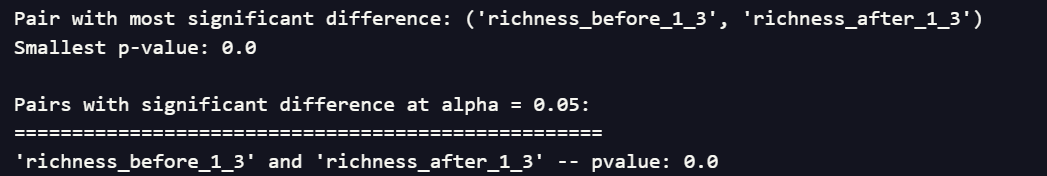
\includegraphics[width=8cm]{keystone_code_small}\label{keystone_code_small}}
	\subfloat[Birds]{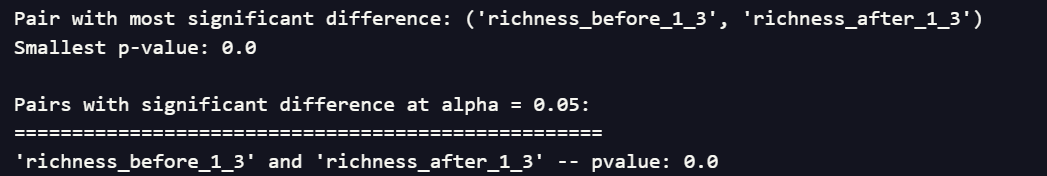
\includegraphics[width=8cm]{keystone_code_small}\label{keystone_code_big}}
	\caption{Test results for mean difference in richness between different time periods}
	\vspace*{-1mm}
\end{figure}
\noindent
In both cases, pairs with the most significant difference were from the period before observations by 1 to 3 years and period after observations by 1 to 3 years. Such results suggested that the occurrence of yellow-breasted bunting could influence species richness of an area.

\subsection{Relationship analysis}
We wanted to present students something different than mere numbers, a more tangible thing which would be helpful to them in understanding the biodiversity in Finland but also how it works. For that purpose, presenting different cases of interactions between different species seemed to serve our purposes. Therefore, we started the groundwork by looking for what kind of interactions and which species we should focus on. Another important aspect there was that those interactions/species should exist in Finland and more specifically dataset that we were using. As concluding relationships just by looking at the data is not really possible, we searched online, compared the results with the dataset we have and concluded that three types of relationships are suitable for our purposes: mutualistic, predatory, and parasitic. For those relationships, we found that from our dataset following combinations were useful:
\begin{itemize}
	\item Mutualistic: Fly agaric mushroom (Amanita muscaria) vs. The baltic pine tree (Pinus sylvestris)
	\item Predatory: Boreal owl (Aegolius funereus) vs. two rodents it hunts -the bank vole (Clethrionomys glareolus) and the field vole (Microtus agrestis)
	\item Parasitic: Downy birch (Betula pubescens) vs The witches broom fungus (Taphrina betulina)
\end{itemize}
\par
Our initial idea after deciding on what to analyze was to use the Pearson correlation coefficient as it is one of the most popular correlation indices and also there were libraries implementing it which means that applying it to our code was not supposed to take much time. Indeed, it did not. We quickly managed to find the data we needed and calculated the Pearson correlation coefficient to our data by the Pandas function. However, it was not very informative. This was mainly because our data was based on the observations and some species were observed more often than others in a way which does not represent the absolute truth regarding the existence of those species in Finland. Therefore, using a correlation function which compares the numbers of species also did not mirror the truth of the relationship between the species. In the end, we decided that it was not good enough to include in our final product.
\par
The next idea was to use a habitat-based approach. In this approach, the main concept was taking advantage of the h3 library we were using. Initially, we transferred all our data into h3 form so that we had a uniform definition of habitat. After that, we decided to create a map for each relationship showing which species exist in each habitat. The goal was that students looking at those maps would be able to understand if the subject species existed in the same areas or if they preferred different habitats. An example of those maps being really useful was the parasitic case. Since the witches broom fungus would only live on the branches of downy birch, in every cell that the witches broom fungus we also had downy birch. That showed a very clear dependence of the witches broom fungus to downy birch. In addition to maps, we also wanted to create bar graphs to present numbers to the students. In our bar graphs, we showed the average number for each species over all cells in different contexts. For example, we showed the average number of one species in all locations in Finland and the average number of the same species in locations that coexisted with the species that is also subject to the relationship. By that, students would be able to understand the relationships more deeply.
\subsection{Conclusions}
After exploring different options for each method, we finally got together and made decisions about how to use different methods in our final product.
\subsubsection{Biodiversity metrics}
Since all of the biodiversity metrics aforementioned provide sufficient and useful information about the diversity of the ecosystem in Finland, we decided to display all of them in our main page.
\subsubsection{MaxEnt model}
In our project, we used Maxent to model the distribution of all bird and mammal species (Biodiversity section) and the plant species $\emph{Ranunculus glacialis}$ (Projects section) based on a set of environmental variables. For a more detailed discussion, please see the Results section.
\subsubsection{Smoothing: Bayesian model}
We used the Dirichlet-multinomial model with uniform prior to infer and visualize biodiversity metrics as shown in Figure 2. 
\par
\begin{figure}[h]
	\vspace*{-3mm}
	\centering
	\subfloat[Actual Richness]{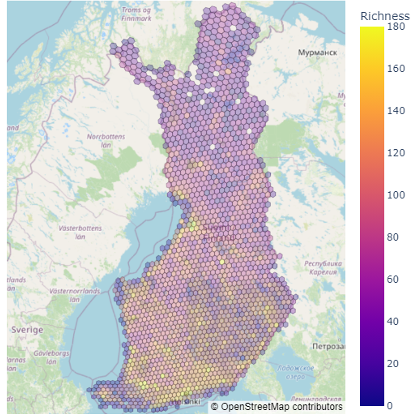
\includegraphics[width=5.5cm]{actual_richness}\label{actual_richness}}
	\subfloat[Inferred Richness]{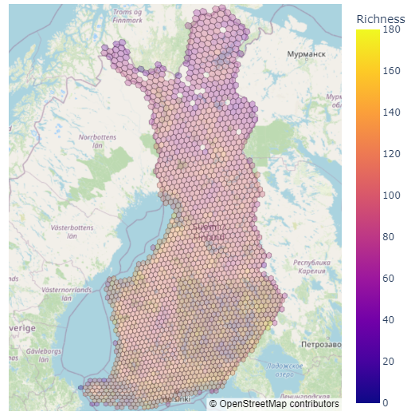
\includegraphics[width=5.5cm]{inferred_richness}\label{inferred_richness}}
	\caption{Richness maps of Finland}
	\vspace*{-1mm}
\end{figure}
\noindent
To calculate species richness using inferred distribution, we only counted species with probabilities higher than a certain threshold because the Bayesian model would not infer probability = 0 for any species. The visualizations showed that inferred distribution yielded higher species richness than that of the actual distribution (observations). This indicated that the model detected many areas with high level of uncertainty and suggested there being more species than observed in such areas.
\par
We encountered 2 major difficulties when applying Bayesian model:
\begin{itemize}
	\vspace*{-1mm}
	\setlength\itemsep{1mm}
	\item Difficulty to evaluate the performance of Bayesian models and optimal parameters as actual species abundance was not available.
	\item Difficulty to implement the calculations on a large dataset, making it not possible to create visualizations on the website.
\end{itemize}
\subsubsection{Keystone species analysis}
The occurrence of yellow-breasted bunting seems to have a positive effect on biodiversity. However, the immediate effect of the species’ disappearance is not recognized.
\par
The study was limited by the low number of data points (areas with observations), diminishing the importance of its results. Furthermore, it would be beneficial to consider different populations (e.g., insects, mammals) to obtain a better overall view. Another direction for future improvements is to use a different method, such as using differences as test statistics to compare with a control group (areas without observations of keystone species).

\subsubsection{Relationship analysis}
Using numbers as they are without any processing to find the relationships between species was not the best idea considering the nature of the dataset that we were using. Even though the Pearson correlation coefficient is a widely praised formula, the natural flaws of our data forced us to explore different ways. Thereafter, we came up with the habitat-based approach where habitats are defined in our usual hexagonal spaces and comparisons are mainly done taking the habitat effects into consideration.
\vspace*{-3mm}
\section{Implementation}
To build the final product, we first did some groundwork so that different facades of the project could have the same uniform look. After doing that, we got together different parts that people had been working independently and built the final website. During the process, we used different tools/libraries and utilized approaches such as precomputation to tackle problems that we faced.
\subsection{Hexagonal gridding}
In order to effectively display the distribution of the biodiversity metrics and the observations of species on a map, we utilized a hexagonal gridding algorithm provided by the h3 library. Essentially, the algorithm finds a way to divide the map into hexagonal cells of a specified area, which is used to group up the observations within each of them. The reason for this specific choice of shape is because the hexagon is among a few shapes that can fill up a certain area without leaving any redundant space, and it can also capture complex distribution (non-linear shape) in the data better due to its more “circular shape”. After performing gridding, we only needed to compute our metrics for each cell and visualize their distribution on the map. You can see an example of it on Figure 3.
\begin{figure}[h]
	\vspace*{-3mm}
	\centering
	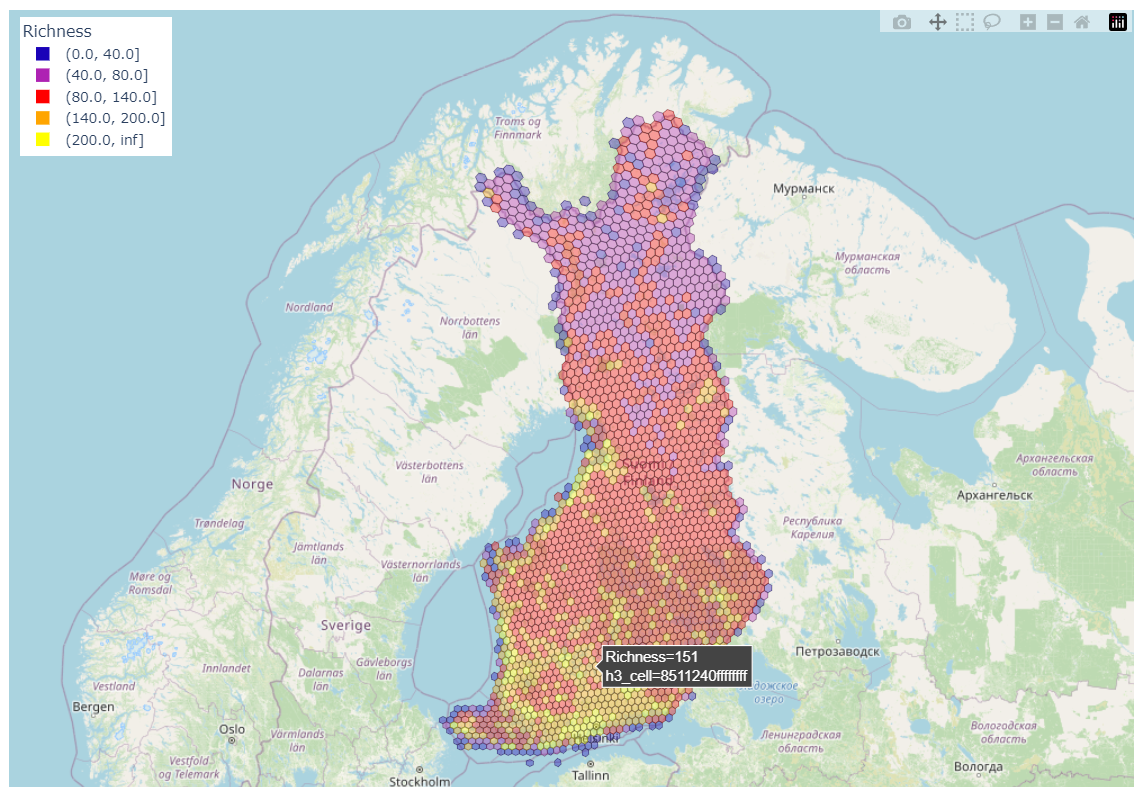
\includegraphics[width=7.46cm]{hexagonal_gridding}\label{hexagonal_gridding}
	\vspace*{-2mm}
	\caption{Example of a hexagonal gridded map to display Richness distribution}
\end{figure}
\vspace*{-5mm}
\subsection{Libraries}
\begin{itemize}
	\setlength\itemsep{1mm}
	\item Plotly: it offers interactive visualizations of various types, from simple bar charts to choropleth maps.
	\item h3: the library contains algorithms that perform hexagonal gridding and neighbour searching, which are central to the groupings of species observation in our data.
	\item Streamlit: the library helps to facilitate the process of building simple websites in Python. Although it only has pre-built components for website building, one can combine still them to design many well-functional and good-looking websites.
	\item Raster, MASS, maptools: Species distribution modeling was performed with the software Maxent [7], which was used as a command line tool. Preparing the input rasters for Maxent was performed with $\texttt{R}$ using the  libraries listed.
\end{itemize}
\subsection{Deployment}
We utilized GitHub as the storage for the scripts and data used for the project, which also includes the website code. Streamlit on the other hand, was chosen to be the hosting site because of its great ease of use while requiring no actual payment. From a simple GitHub integration procedure, Streamlit helped us conveniently load large data sets and resources into the server smoothly.
\subsection{Precomputation of data}
One major problem we encountered during deployment was finding a way to load various complex and memory-heavy computations to the website. Streamlit, though was a very good tool to build websites, offered only 1GB in memory usage. At the time, all of the computations needed for the biodiversity metrics and visualizations took up to 4GB of memory, which is four times over the limit. In order to resolve this, we came up with a plan to precompute every data and every visualization we wanted to have on the website. After that, we would form a file look-up system to only load the precomputed resources in, therefore completely mitigating the need to compute anything on the website.
\par
The method would require extra work to compute everything beforehand, which took a quite significant amount of time to complete given the large size of the data and the complexity of the metrics computation. Nevertheless, this plan was the best option we had when working with such large data, and we finally were successful in loading all the resources into Streamlit later.
\section{Results}
On our website, we tried to take advantage of what Streamlit provides to us as much as we can. To avoid having a tangled view which would make looking around and exploring the data harder for users, we decided to divide our content into 4 different tabs: Biodiversity, Relationships, Projects, and About. All of the tabs focus on different sides of the product and provide different ways for users to learn about biodiversity in Finland. As can be seen in Figure 4, users can switch between different tabs of the website on the top bar.
\begin{figure}[h]
	\vspace*{-2mm}
	\centering
	{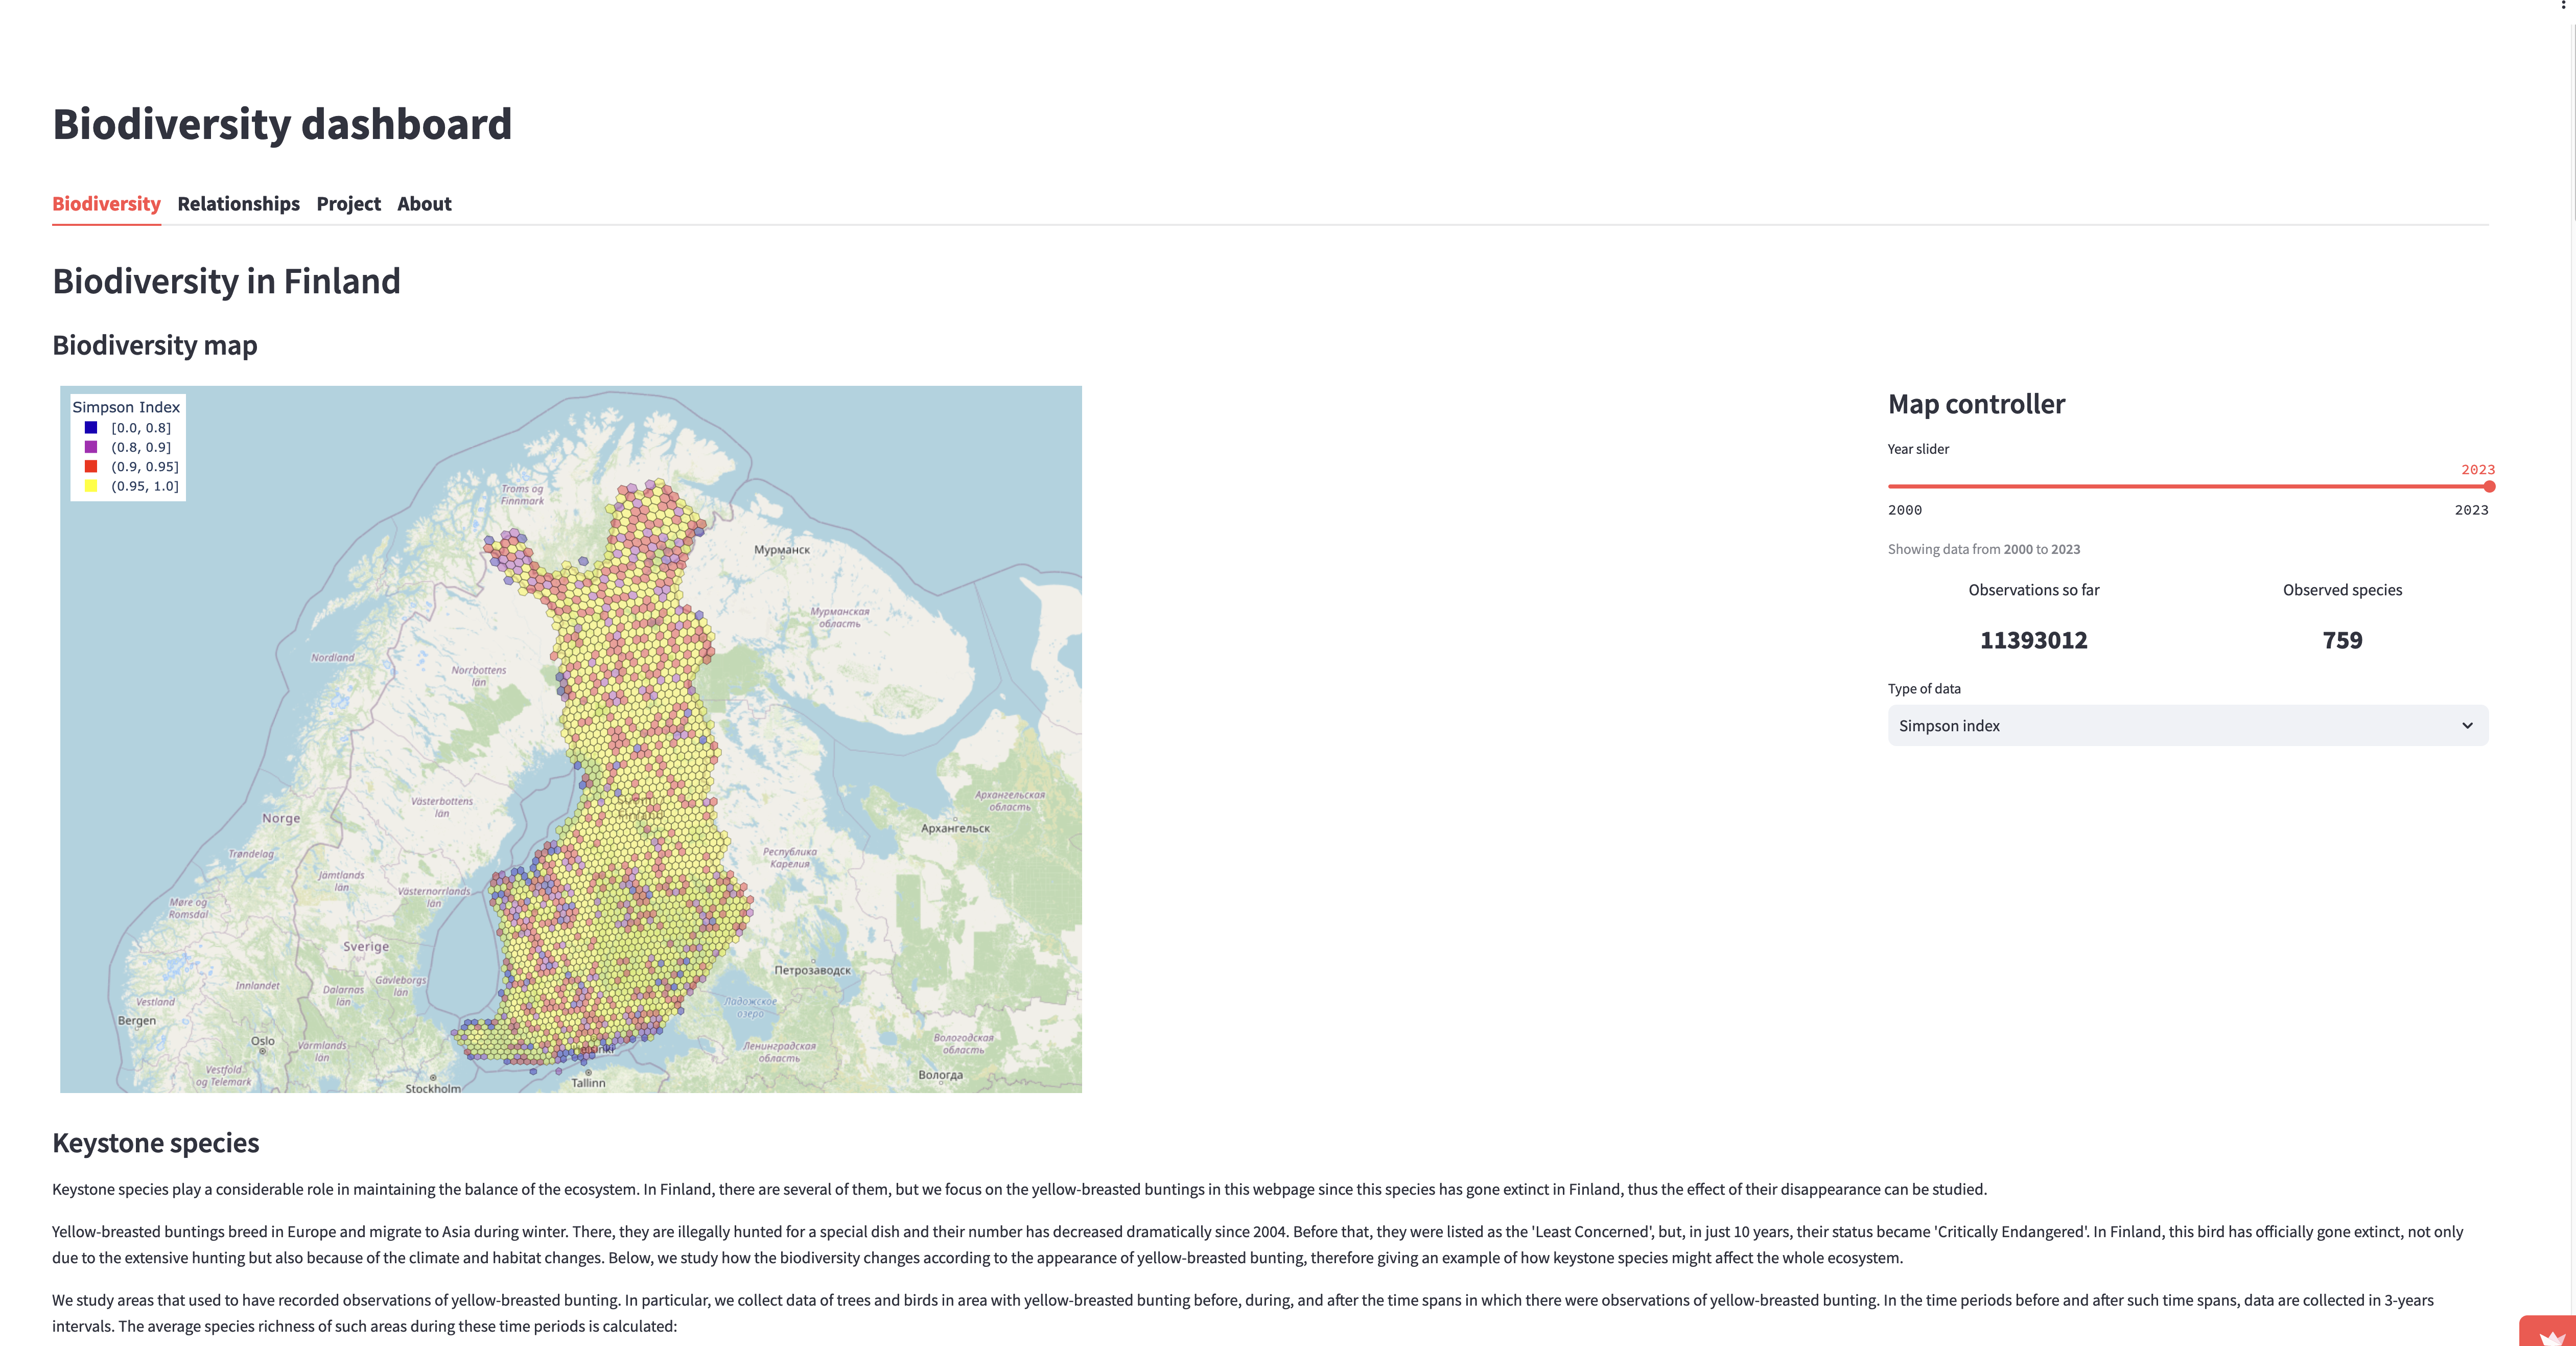
\includegraphics[width=10cm]{landing_page}\label{landing_page}}
	\vspace*{-2mm}
	\caption{Outline of the website}
	\vspace*{-5mm}
\end{figure}
\subsection{Biodiversity page}
The biodiversity page is the main page where we present facts about the biodiversity in Finland. As shown in Figure 4, the page starts with a map and two control buttons: A slider for years to include and a dropdown menu to select a metric to display on the map. By adjusting the slider, users can choose up until which year they would like to include data and from the dropdown menu, they can choose the biodiversity metrics that we introduced before to display it on a map. Hence, the map is totally customizable and users have the freedom to explore different sides of the data on a map. Later on the page, we dive more into keystone species and the MaxEnt model.
\subsubsection{Keystone species analysis}
In Figure 5, we visualized the individual effect of yellow-breasted bunting on each area during 3 periods which had significant mean differences: period before observations by 1 to 3 years, period with observations, and period after observations by 1 to 3 years.
\begin{figure}[h]
	\vspace*{-2mm}
	\centering
	\subfloat[Trees]{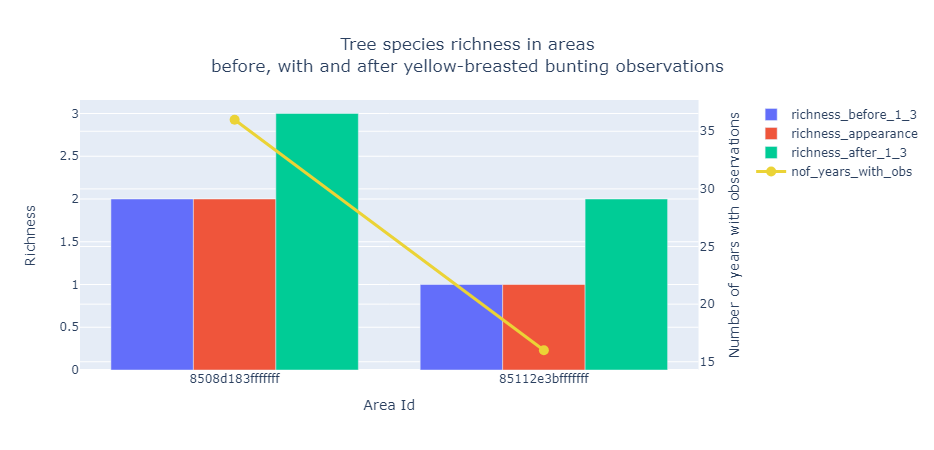
\includegraphics[width=8.5cm]{keystone_graph1}\label{keystone_graph_1}}
	\subfloat[Birds]{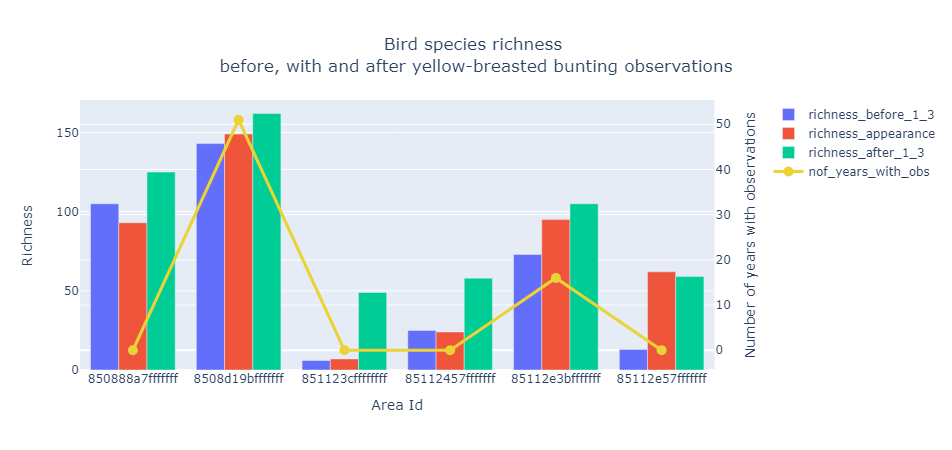
\includegraphics[width=8.5cm]{keystone_graph2}\label{keystone_graph_2}}
	\vspace*{-2mm}
	\caption{Species richness of trees and birds before, with, and after records of keystone species}
	\vspace*{-5mm}
\end{figure}
\subsubsection{MaxEnt model}
In this section, we use Maxent to model the species richness of birds and mammals based on a set of 19 bioclimatic variables (BIO1 - BIO19) provided by WorldClim [8]. For each species, we extracted the observation locations of that species and fed them into Maxent together with the 19 environmental grids. A bias file [5] was also included to account for sampling bias. The result is the probability of presence $p$ of a species in each grid cell, to which we applied a threshold of 0.5 to infer the binary labels “present” ($p >$ 0.5) or “not present” ($p \leq$ 0.5). We then counted the number of species inferred as present in each grid cell and obtained the species richness value. Finally, we calculated the Pearson’s correlation between each bioclimatic variable and species richness to identify the variables that are highly correlated with species richness. The results for birds are given in Figure 6.
\par
\begin{figure}[h]
	\vspace*{-3mm}
	\centering
	\subfloat[Richness]{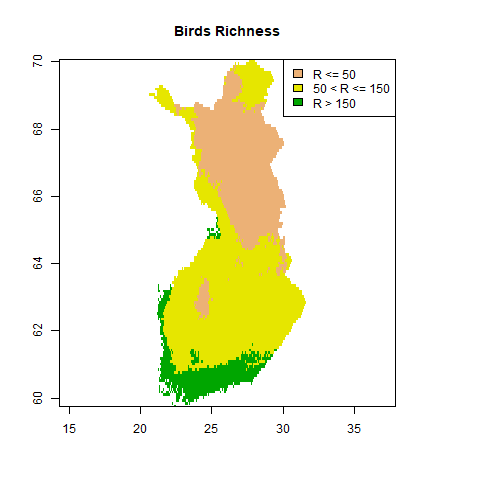
\includegraphics[width=6cm]{birds_richness}\label{birds_richness}}
	\subfloat[Effect of bioclimatic variables]{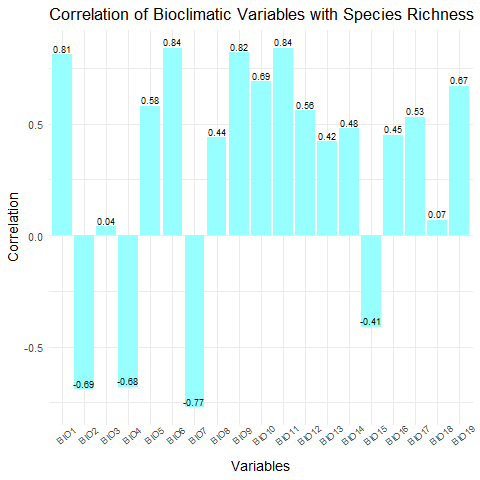
\includegraphics[width=6cm]{birds_corr}\label{birds_corr}}
	\vspace*{-2mm}
	\caption{Birds and bioclimatic variables}
\end{figure}
We discovered that bird richness is strongly positively correlated (corr $>$ 0.7) with BIO11 (Mean Temperature of Coldest Quarter), BIO6 (Min Temperature of Coldest Month), BIO9 (Mean Temperature of Driest Quarter), BIO1 (Annual Mean Temperature). Meanwhile, bird richness is strongly negatively correlated (corr $< -0.7$) with BIO7 (Temperature Annual Range). The results for mammals are given in Figure 7.
\par
\begin{figure}[h]
	\vspace*{-3mm}
	\centering
	\subfloat[Richness]{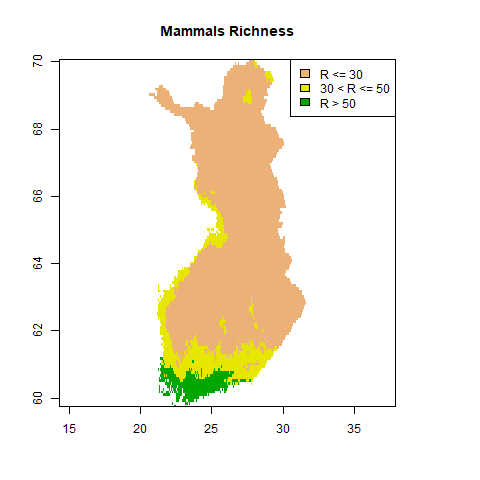
\includegraphics[width=6cm]{mammals_richness}\label{mammals_richness}}
	\subfloat[Effect of bioclimatic variables]{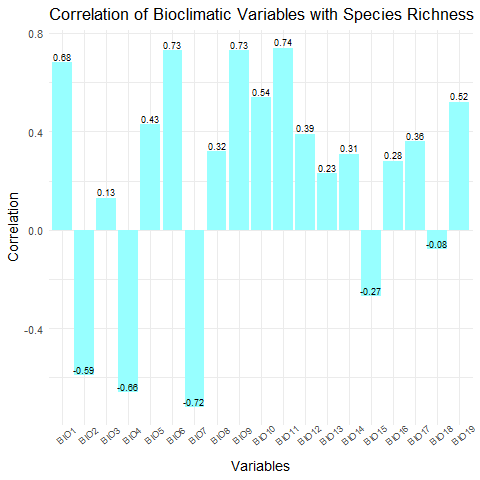
\includegraphics[width=6cm]{mammals_corr}\label{mammals_corr}}
	\vspace*{-2mm}
	\caption{Mammals and bioclimatic variables}
\end{figure}
We discovered that mammals richness is strongly positively correlated (corr $>$ 0.7) with BIO11 (Mean Temperature of Coldest Quarter), BIO6 (Min Temperature of Coldest Month), BIO9 (Mean Temperature of Driest Quarter). Meanwhile, mammals richness is strongly negatively correlated (corr $< -0.7$) with BIO7 (Temperature Annual Range).
\subsection{Relationships page}
In the relationships tab, we wanted to have a compact design and show everything to students clearly without providing an excessive amount of information that might be confusing. With that in mind, we decided to provide short textual information about the relationship type that they are working on, the species chosen, and what the visualizations are about. We also had hyperlinks to Encyclopædia Britannica in case they would like to learn more about the topic. [9, 10]
\par
To make the design neater, we put different types of relationships on different pages that they can change from the dropdown menu on the top. That saved us space on the screen so that we didn’t need to put all the different relationships on the same page, which would not only create an oversupply of information that distracts the users but also would slow down the website due to an increase in number of elements that it tries to load. You can see the general outline of Relationships page on Figure 8.
\newpage
\begin{figure}[h]
	\vspace*{-3mm}
	\centering
	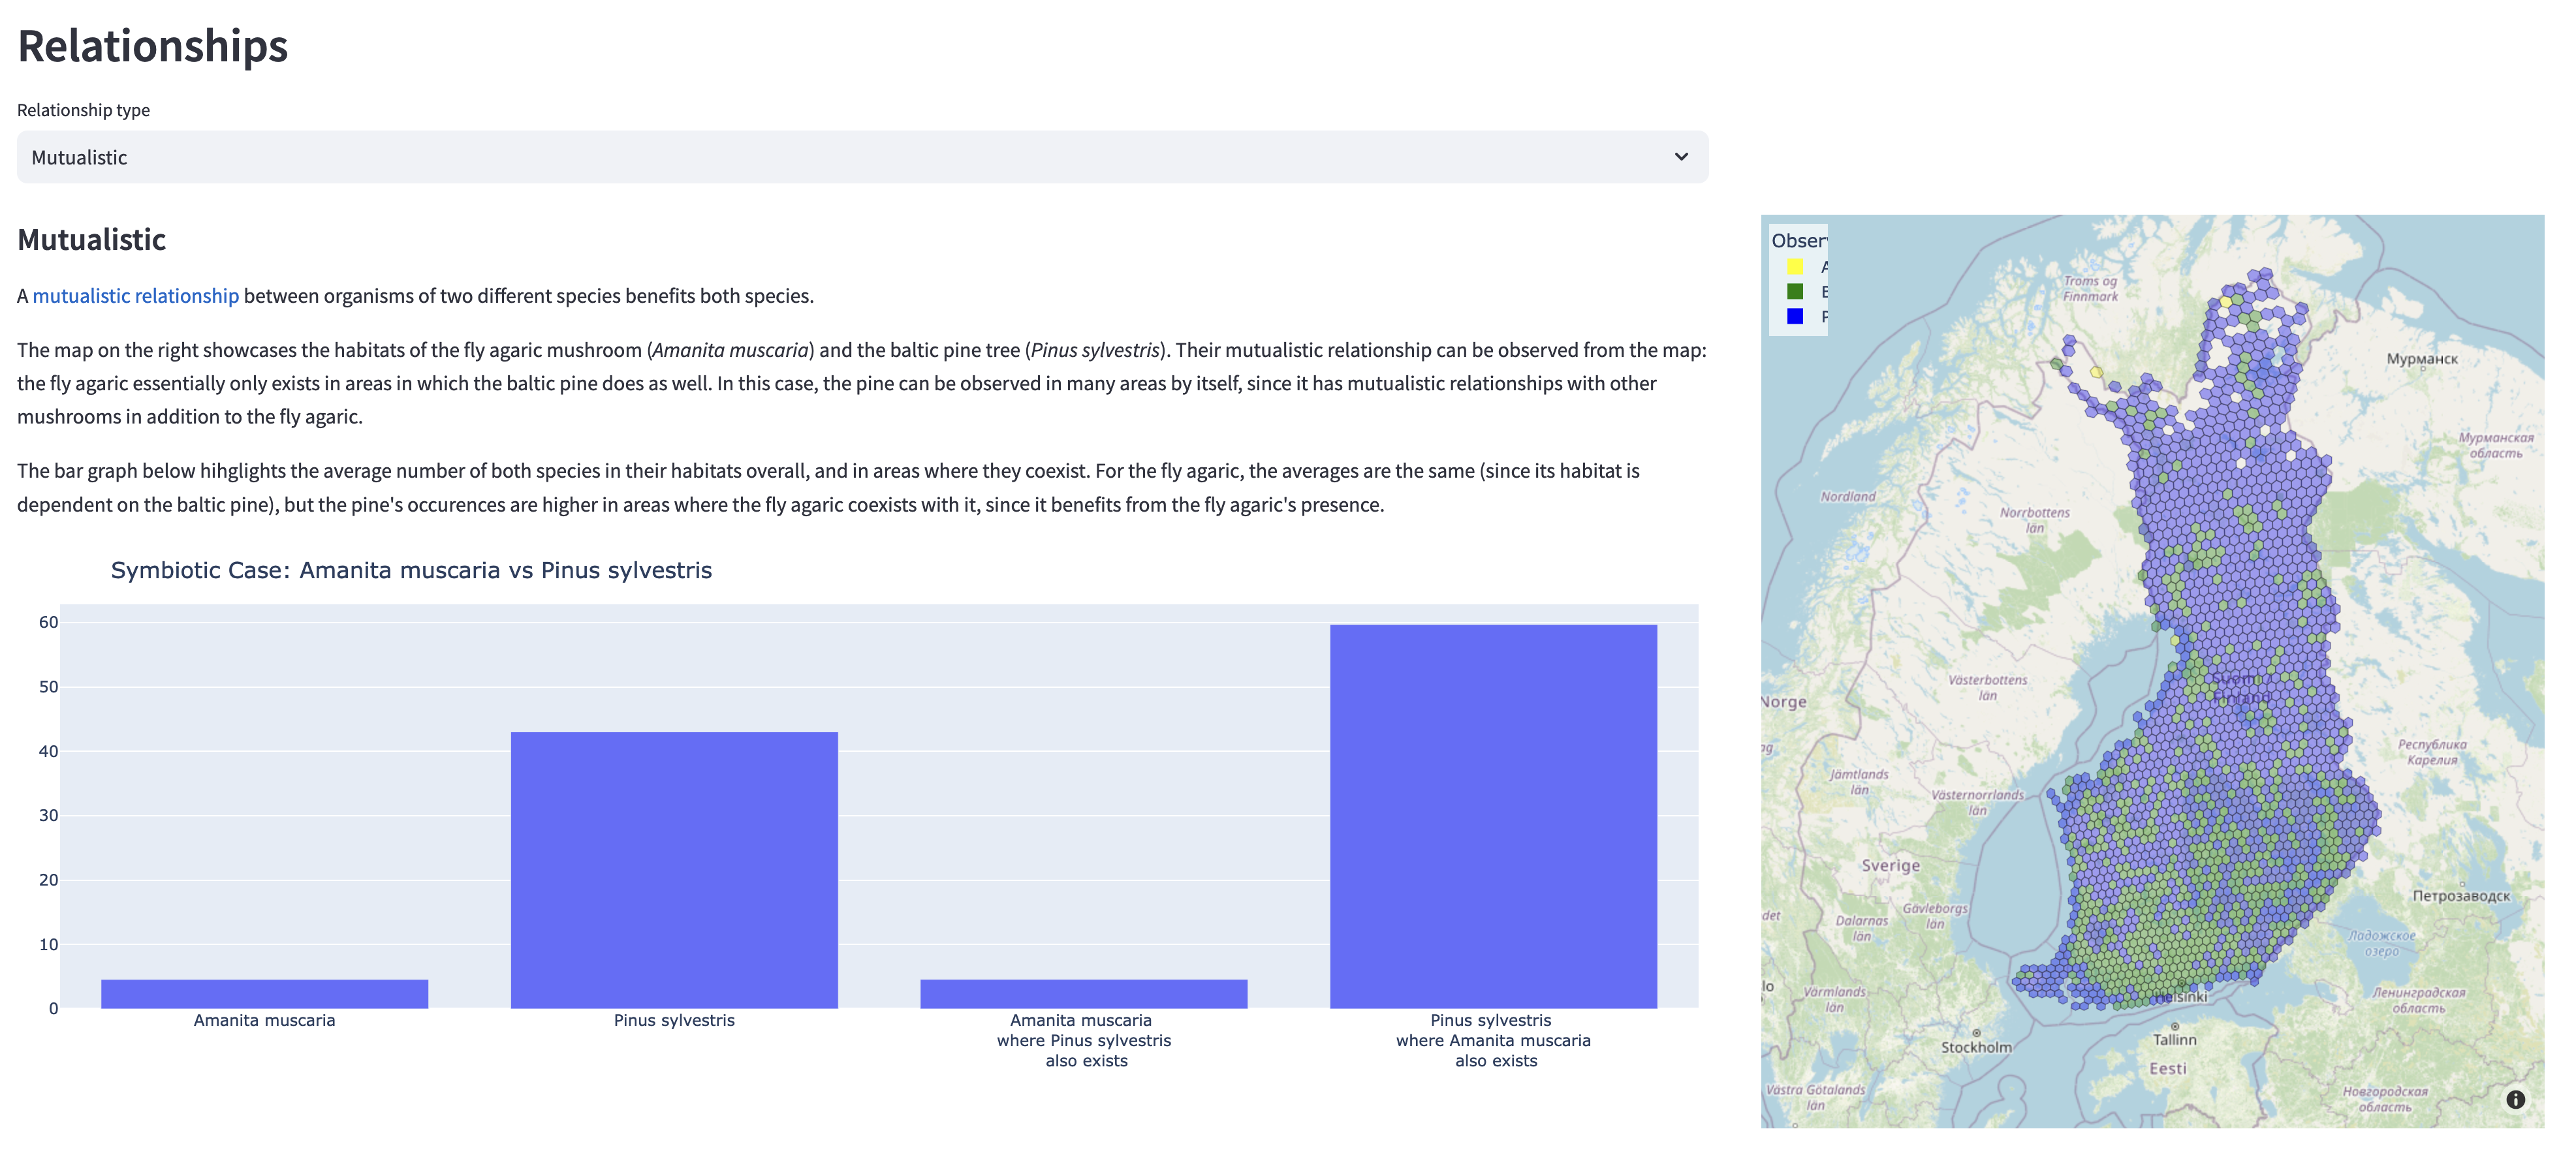
\includegraphics[width=10cm]{relationships_page}\label{relationships_page}
	\vspace*{-2mm}
	\caption{Relationships page}
	\vspace*{-2mm}
\end{figure}
Maps presented in this section are built in a similar way to maps in the biodiversity section. We used the h3 library to obtain the same hexagonal division. The main difference is, here the main interest was not on the number of the species but it was on in which locations which species exist. By that, we were aiming that students would be able to learn more about the habitat preferences of species subject to the relationships. For example in the parasitic case, this was quite informative since the parasite (the witches broom fungus) only lives in locations where the host (downy birch) also lives. This shows a clear dependence of parasite to host and it would be useful to students to understand what such dependences might suggest.
\par
In the bar graphs, we decided to tell more about the numbers with the same habitat-based approach. Here, the first two columns show the average number of species 1 and species 2 over all the locations in Finland, respectively. To make comparisons, we decided to create the third and fourth columns showing the average number of species 1 and species 2 over the locations where they exist together, respectively. With that, students would be able to how the existence of one species is affected by the existence of the other species on average.
\subsection{Projects page}
To give students things to work on and facilitate active learning, we decided to build some projects on the data that we have which students can use to explore more about the biodiversity in Finland. Every project is unique and tries to touch on different sides of the data.
\par
In projects, we provide students with some visualizations and instructions to go through that might be helpful to them to start. In addition to that, we also provide the data used in building the project in CSV format so that students can download and experiment with the data as well.
\par
The Projets tab is structured in dropdown buttons to make it possible to have three projects in a single tab but still keep them separate. The outline of the Projects tab is shown in Figure 9.
\begin{figure}[h]
	\vspace*{-1mm}
	\centering
	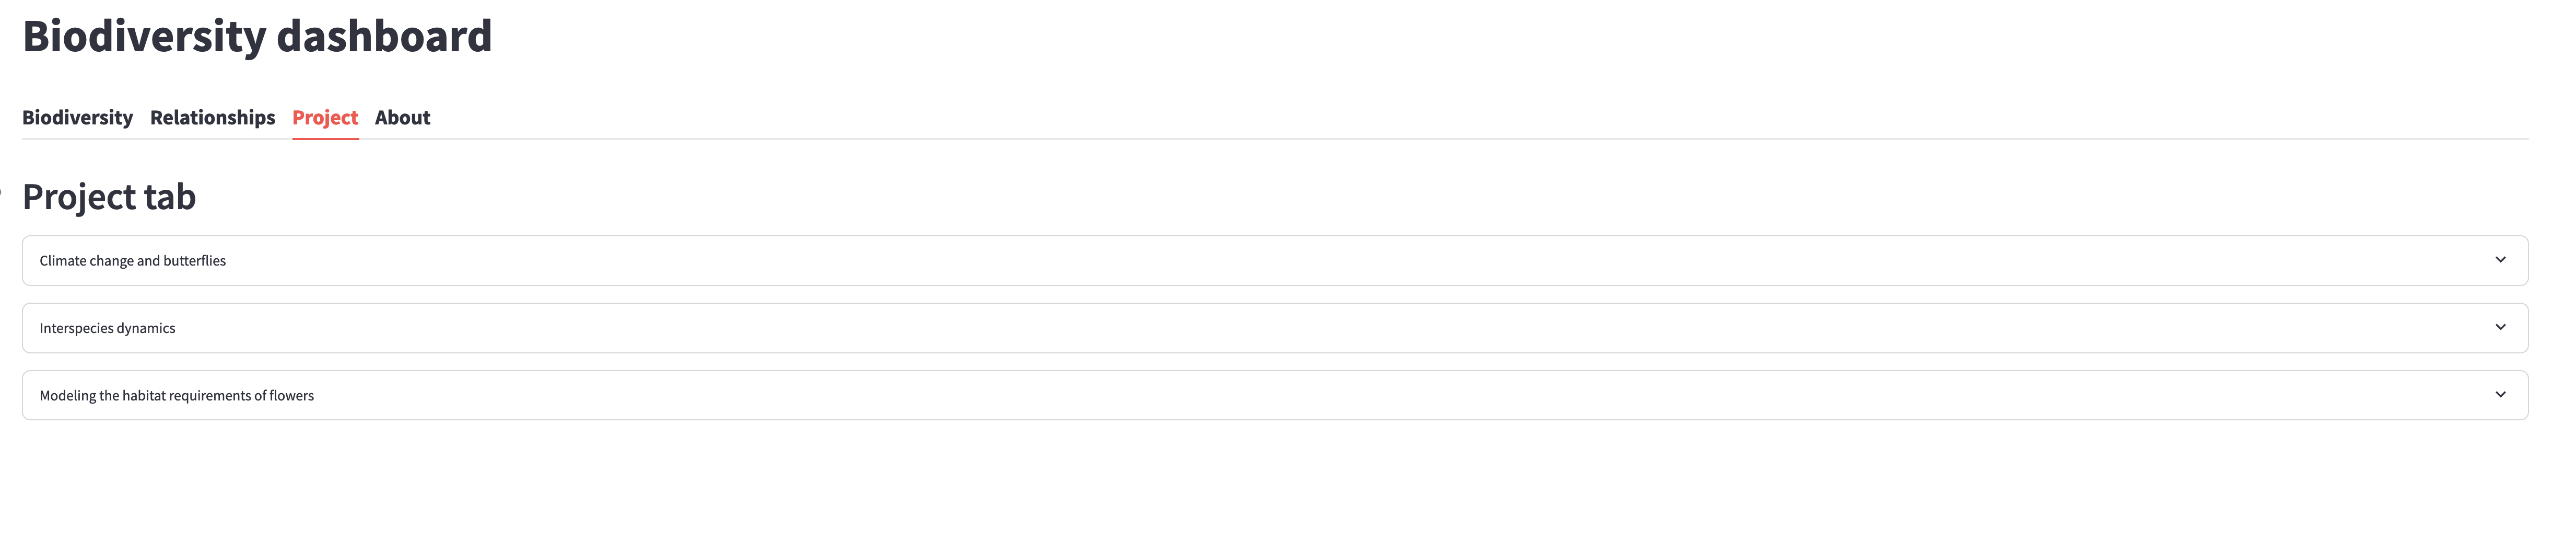
\includegraphics[width=18cm]{projects_page}\label{projects_page}
	\vspace*{-2mm}
	\caption{Projects page}
\end{figure}
\subsubsection{Climate change and butterflies}
In this project, our goal was to make students think about how biodiversity is affected by environmental factors. Butterflies are known to be very sensitive to the surrounding environment and climate change is one of the most important phenomena of recent times. Here, students are given instructions to look at the map, change the year to analyze on the slider on the right side and download the data if they wish to think more about the effects of climate change on butterflies. In addition to that, they were instructed to think about why that specific type of butterfly (Gonepteryx rhamni) is more concentrated in the southern parts of Finland. The visualzations of the projects are provided in Figure 10.
\begin{figure}[h]
	\vspace*{-3mm}
	\centering
	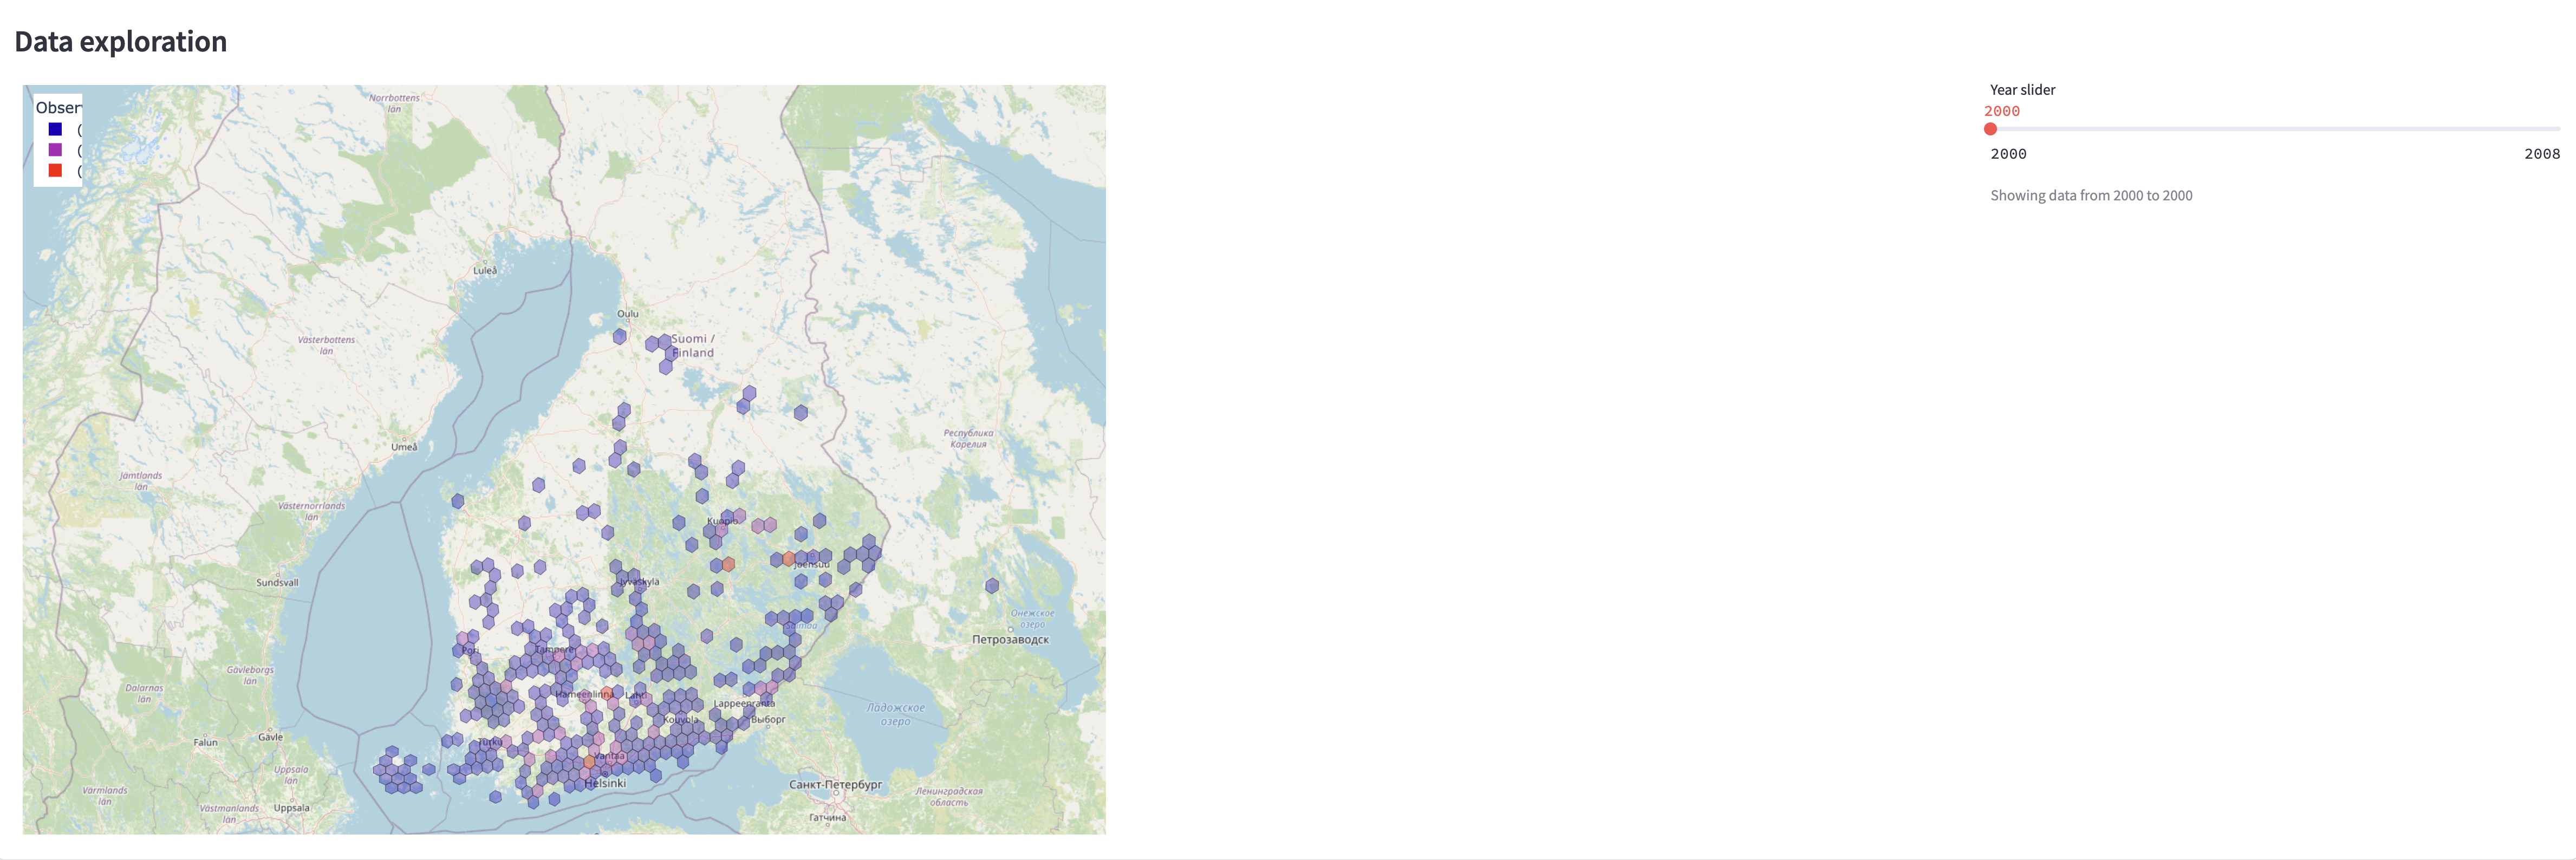
\includegraphics[width=15cm]{climate_butterflies}\label{climate_butterflies}
	\vspace*{-2mm}
	\caption{Visualizations for climate change and butterflies project}
\end{figure}
\newpage
\subsubsection{Interspecies dynamics}
In this project, students are encouraged to analyze the relationship between a mushroom (Cantharellus cibarius) and a tree (Pinus sylvestris). This project topic is designed to be a more thought-provoking version of the relationships page. In the relationships page, we explained to students different kinds of interspecies relations with examples and visualizations. Here, students are expected to have the same methodology of thinking using the same kind of visualizations to find out what the relationship here. They are also encouraged to search the web and download the data to reveal more about it. The visualzations of the projects are provided in Figure 11.
\begin{figure}[h]
	\centering
	\subfloat[Map]{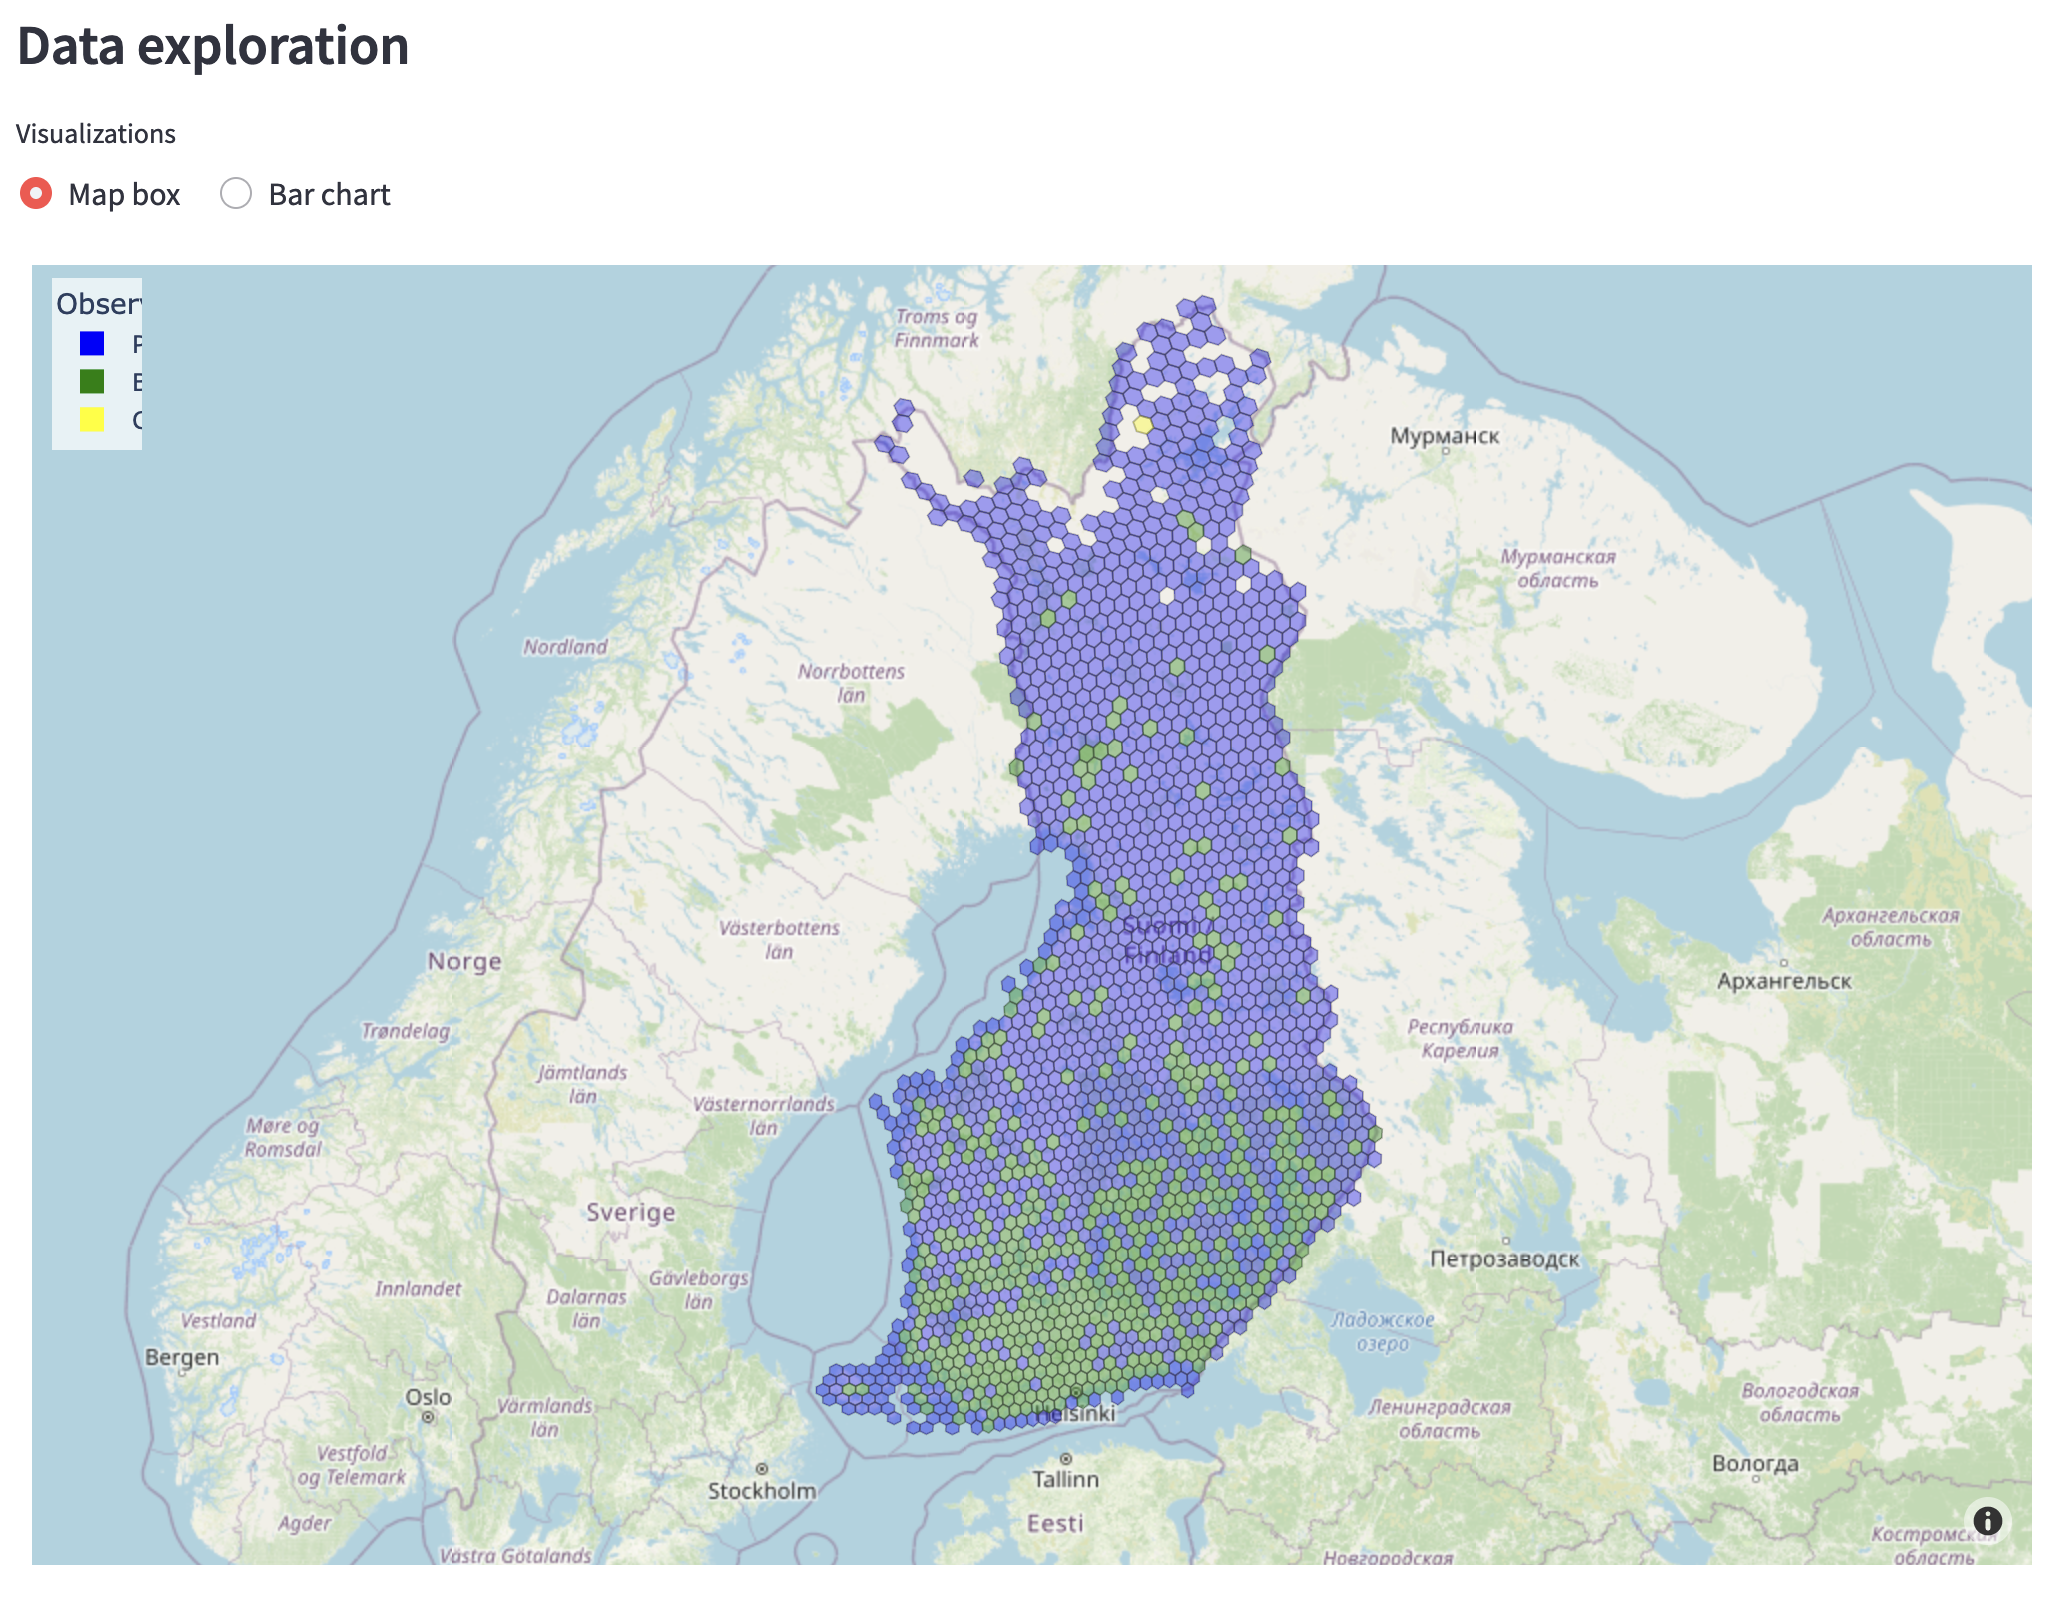
\includegraphics[width=7.5cm]{interspecies_map}\label{interspecies_map}}\\
	\subfloat[Bar graph]{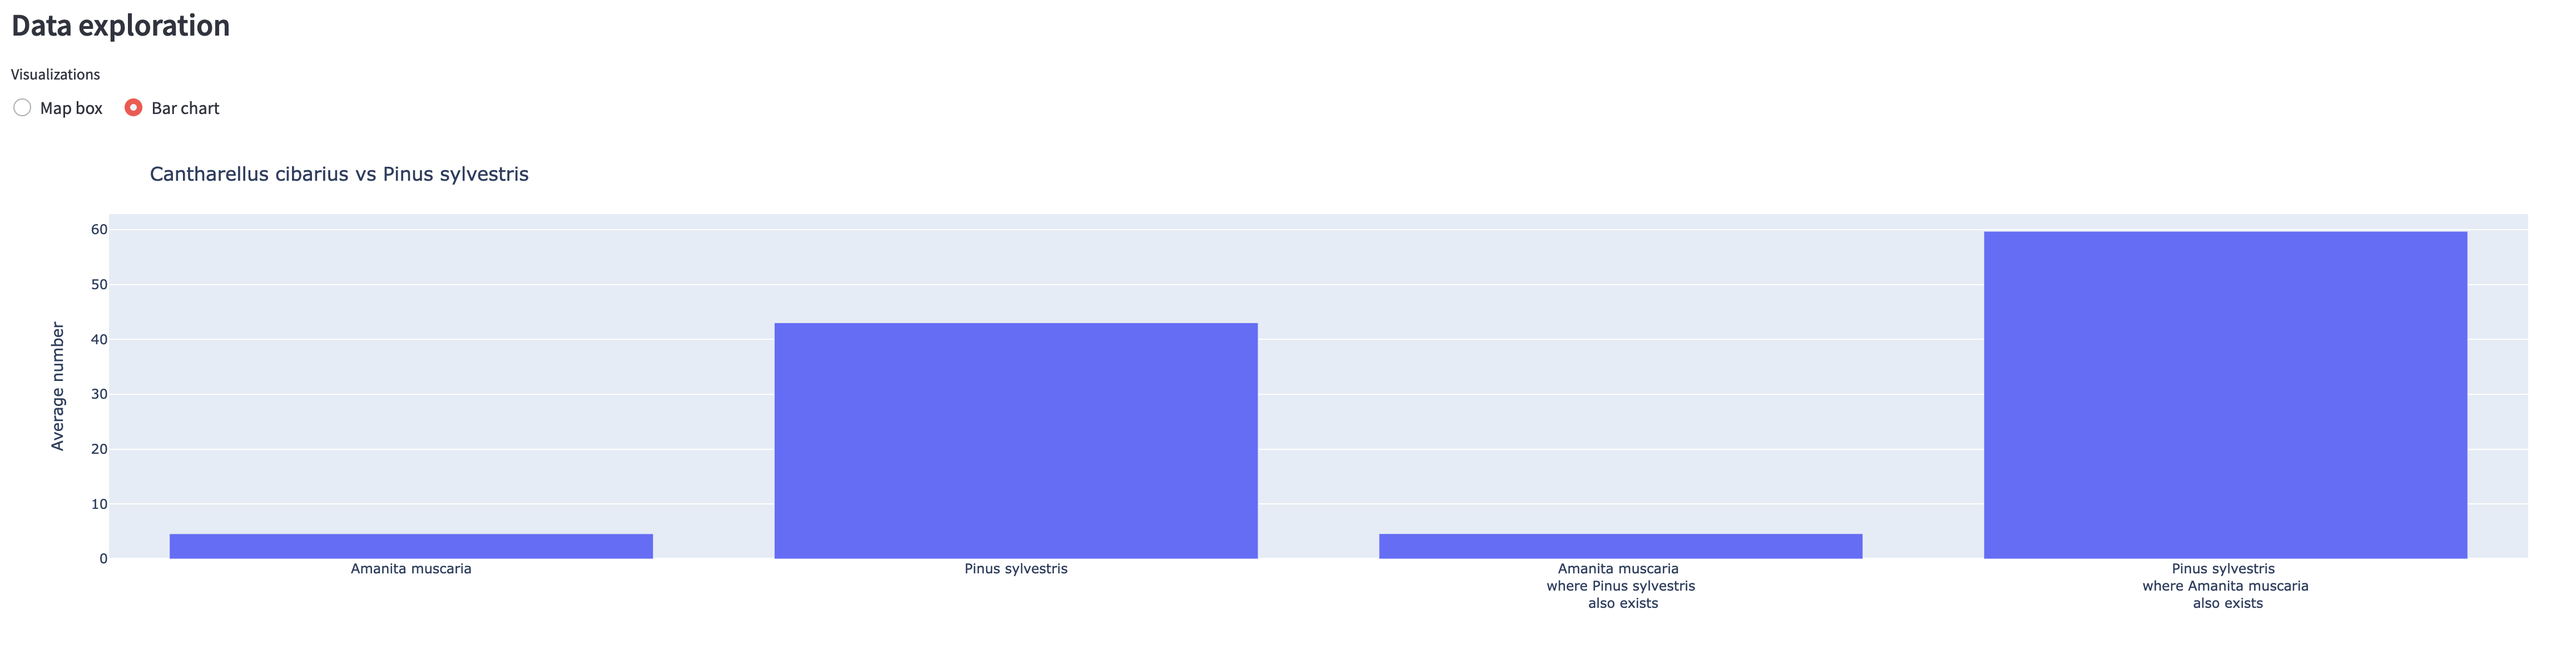
\includegraphics[width=11cm]{interspecies_bar}\label{interspecies_bar}}
	\vspace*{-2mm}
	\caption{Visualizations for interspecies dynamics project}
\end{figure}
\subsubsection*{Modeling the habitat requirements of \emph{Ranunculus glacialis}}
$\emph{Ranunculus glacialis}$ is a rare, endangered plant species in Finland. In this section, we first modeled the distribution of $\emph{Ranunculus glacialis}$ based on annual average temperature, annual precipitation, and elevation. We then plotted the distribution map and the maps of the three environmental variables, and asked the students to make inferences on the habitat requirements of $\emph{Ranunculus glacialis}$ with regard to each of the three environmental variables. The plots are given in Figure 12.
\newpage
\begin{figure}[h]
	\vspace*{-3mm}
	\centering
	\subfloat[Ranunculus glacialis]{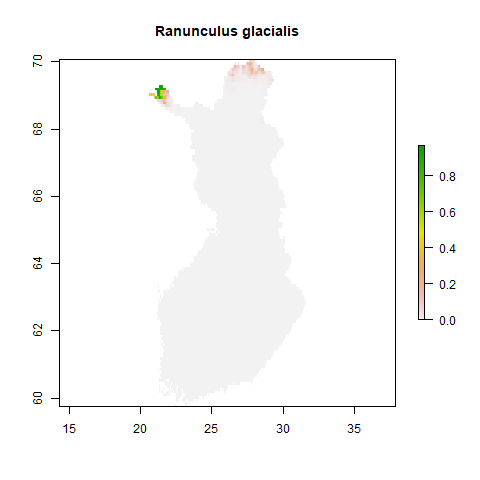
\includegraphics[width=6.4cm]{ranunculus}\label{ranunculus}}
	\subfloat[Mean temperature]{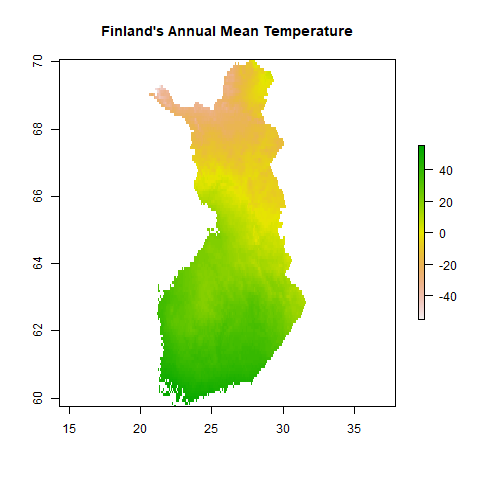
\includegraphics[width=6.4cm]{temperature}\label{temperature}}
	\vspace*{-10mm}
\end{figure}
\begin{figure}[h]
	\centering
	\setcounter{subfigure}{2}
	\subfloat[Annual precipitation]{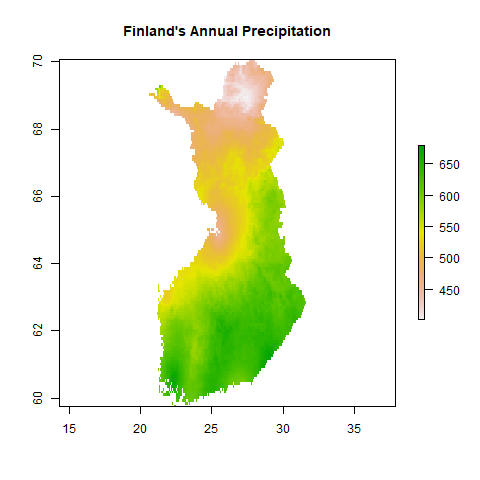
\includegraphics[width=6.4cm]{precipitation}\label{precipitation}}
	\subfloat[Elevation]{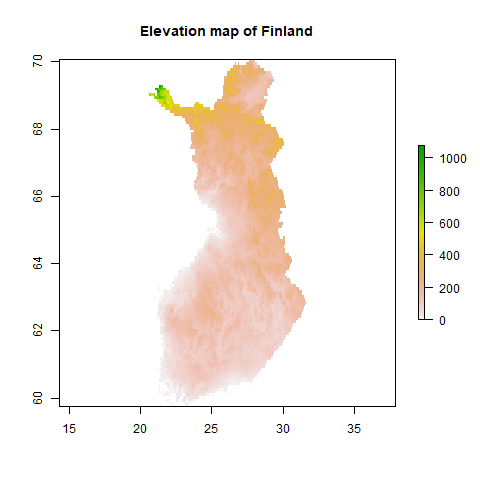
\includegraphics[width=6.4cm]{elev}\label{elevation}}
	\vspace*{-2mm}
	\caption{Visualizations for habitat requirements project}
\end{figure}
\vspace*{-5mm}
\subsection{About page}
In our webpage, we included a tab called ‘About’ providing an overview of our methods and a guideline to utilize the information presented on the website. Our data source was from laji.fi and the data points were observations reported by people, so they were not the accurate number of species individuals. Because this problem was related to some ethical issues, we wanted to state it beforehand. We briefly introduced the metrics calculated in the Biodiversity tab, together with instructions on how to interpret those numbers, and a general outline of the tab. For the Relationships tab, the types of relationships were also presented. In addition to those tabs, we also had a Project tab that we thought would be better for readers to visit the tab itself for detailed instructions.
\begin{figure}[h]
	\centering
	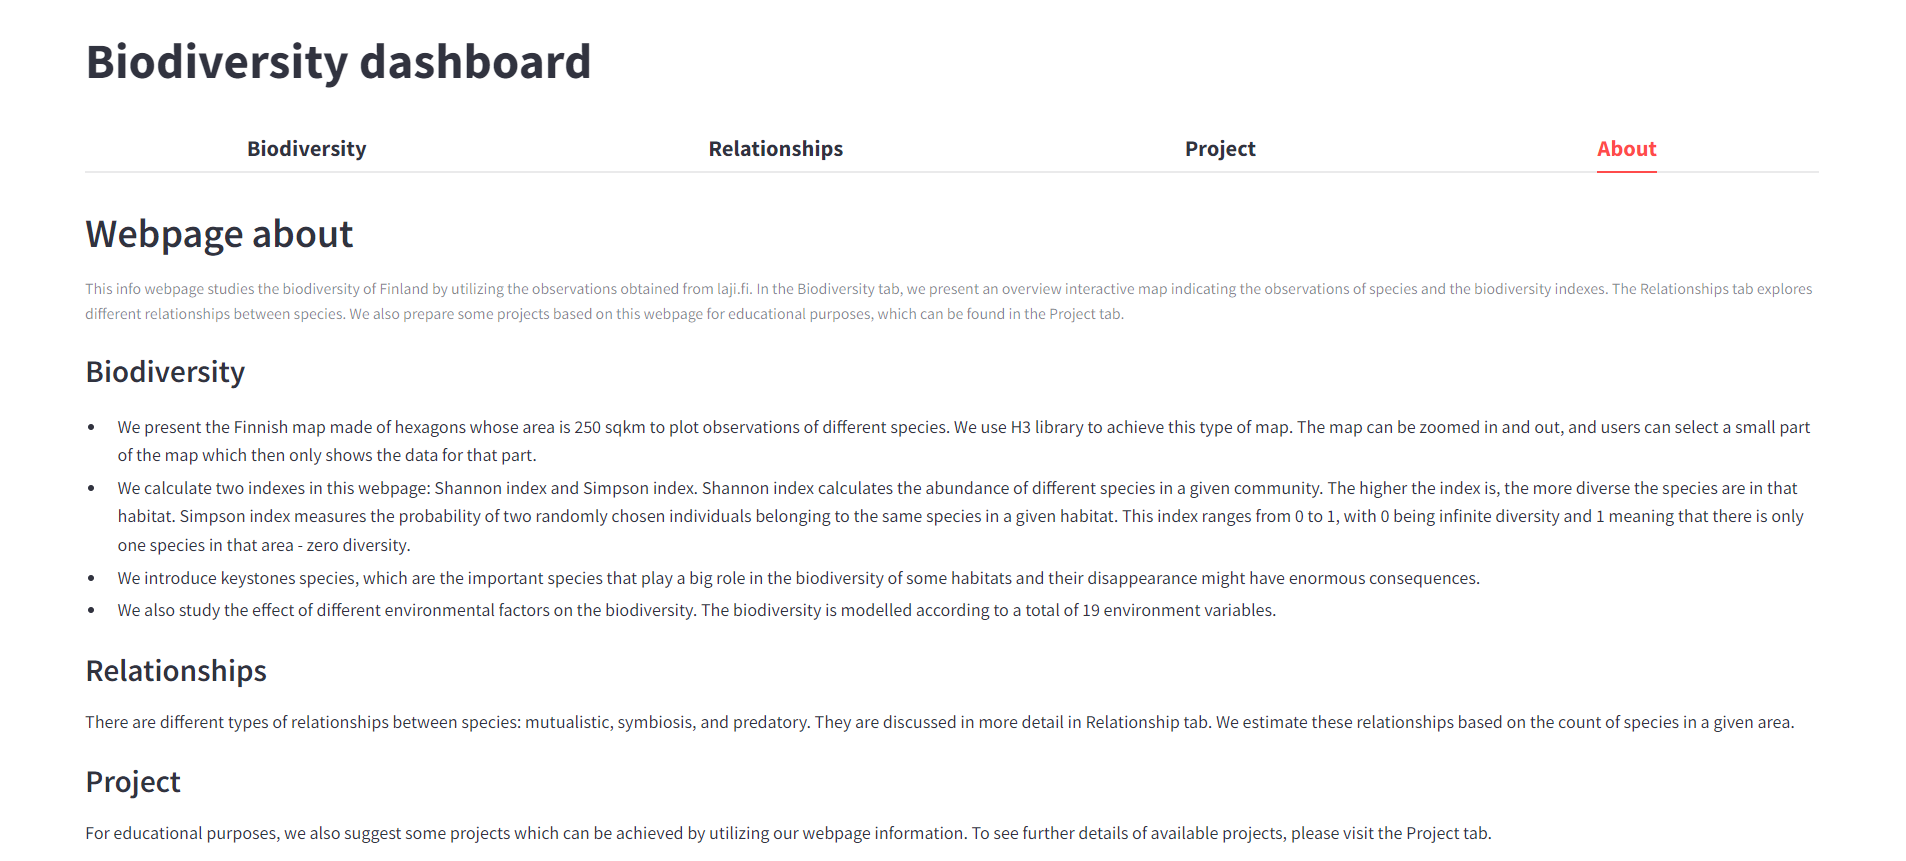
\includegraphics[width=10cm]{about_page}\label{about_page}
	\vspace*{-2mm}
	\caption{About page}
\end{figure}
\newpage
\section{Ethical issues}
The project’s premise implies very few ethical issues, if any. We did not have to work with any sensitive or personal data. On top of that, all endangered species are hidden on laji.fi, thereby we were not able to access it. That made it impossible to accidentally disclose information about endangered species to the general public, including potential bad actors.
\par
Nevertheless, one of our considerations was the accuracy of the data and its delivery. We had to present the information to high-school students who might not be particularly knowledgeable about the topics of biodiversity, biology, and data science. That made us more attentive to the wording and the ways we demonstrated our findings so that the judgment formed by the students would be as unbiased as possible.
\section{Lessons learned}
Starting the project posed certain challenges. It was hard to understand what to begin with, as we had to start with a blank slate and more than forty million data points that contained all observations of living species that have been made and recorded in Finland. Moreover, we encountered problems with downloading data in somewhat reasonable amounts, as the API of laji.fi had quite a low limit for a single download. It was circumvented by a simple algorithm, although it still required a lot of time to download all the data we needed as some latency constraints were present.
\par
One of the significant realizations was that a sound proof of concept could be achieved with a smaller subset of data. Despite having access to approximately 40 million data points, the project effectively utilized about 15 million of them. This approach demonstrated that smaller, more manageable datasets could still yield significant insights and results that would result in a viable product.
\par
Another important realization was about precomputation. Precomputing data that we were intending to display on the web page turned out to be really helpful. By processing data beforehand, our team was able to provide a more seamless and efficient interface for end-users. That allowed us to successfully deploy the project using limited resources that we had at hand.
\section{Conclusion and future prospects}
In conclusion, we could say that the project was carried out successfully despite challenges and bottlenecks we faced. Moreover, we believe that the current implementation, although sufficient in itself, can be expanded further to constitute even more thorough implementation of the customer’s task.
\par
Looking forward, the project aims to integrate live data, potentially connecting with platforms like laji.fi. This would allow for a dynamic representation of data, enabling users to observe real-time changes in maps and other data visualizations.
\par
Another objective is to increase user interactivity by introducing a bit more advanced features like tooltips. These would supplement the existing informational resources, such as the 'About' page, thus providing users with a more engaging experience.
\par
Last but not least, the goal to change our data storage and processor seems to be important. Currently, the project relies on local CSV files for data storage and utilizes precomputed graphs uploaded to the website. Future iterations plan to streamline this process by integrating a database system. This would not only enhance efficiency but also improve the scalability and maintainability of the project infrastructure. Which would be particularly important if we were to incorporate live data.

\section{Divison of tasks}
Ilya worked on project management and facilitation, maintaining communication with the client, projects  scaffolding, and reporting. Hung dealt with Streamlit implementation and hosting of the project, creating a script to fetch data from laji.fi, hexagonal mapping, reporting. Linh implemented the about page of the website, data processing, keystone species exploration, and reporting. Aaron researched relationships of the species, hexagonal mapping, interspecies dynamics project, reporting. Kerkko worked on keystone species exploration, butterfly and climate change project, and reporting. Chau carried out environmental variables analysis, geostatistics, biodiversity metrics, habitat of flowers project, and reporting. Behram relationships of the species, interspecies dynamics project, and reporting. Finally, Nghi researched biodiversity metrics, smoothing methods with Bayesian methods, keystone species, and did reporting.
\newpage
\section{References}
\renewcommand{\section}[2]{} %Removing the references title

\begin{thebibliography}{11}
	\bibitem{laji.fi}
	laji.fi [WWW Document]. URL \url{https://laji.fi/} (accessed 6.12.23).
	
	\bibitem{maxent}
	Phillips, S.J., Anderson, R.P., Schapire, R.E., 2006. Maximum entropy modeling of species geographic distributions. Ecological Modelling 190, 231–259.
	
	\bibitem{elith}
	Elith*, J., H. Graham*, C., P. Anderson, R., Dudík, M., Ferrier, S., Guisan, A., J. Hijmans, R., Huettmann, F., R. Leathwick, J., Lehmann, A., Li, J., G. Lohmann, L., A. Loiselle, B., Manion, G., Moritz, C., Nakamura, M., Nakazawa, Y., McC. M. Overton, J., Townsend Peterson, A., J. Phillips, S., Richardson, K., Scachetti‐Pereira, R., E. Schapire, R., Soberón, J., Williams, S., S. Wisz, M., E. Zimmermann, N., 2006. Novel methods improve prediction of species’ distributions from occurrence data. Ecography 29, 129–151.
	
	\bibitem{maxenttut}
	Phillips, S., 2010. A Brief Tutorial on Maxent. Network of Conservation Educators and Practitioners, Center for Biodiversity and Conservation, American Museum of Natural History. Lessons in Conservation 3, 108-135.
	
	\bibitem{sdm}
	SDMtoolbox. SDMtoolbox: a python-based ArcGIS toolbox for evolution and ecology [WWW Document]. URL \url{http://www.sdmtoolbox.org/} (accessed 5.12.23).
	
	\bibitem{barber}
	Barber, R.A., Ball, S.G., Morris, R.K.A., Gilbert, F., 2022. Target‐group backgrounds prove effective at correcting sampling bias in Maxent models. Diversity and Distributions 28, 128–141.
	
	\bibitem{maxentweb}
	American Museum of Natural History. Maxent is now open source! [WWW Document]. URL \url{https://biodiversityinformatics.amnh.org/open_source/maxent/} (accessed 5.12.23).
	
	\bibitem{worldclim}
	WorldClim [WWW Document]. URL \url{https://www.worldclim.org/} (accessed 5.12.23).
	
	\bibitem{symbiosis}
	Symbiosis [WWW Document]. URL \url{https://www.britannica.com/science/symbiosis} (accessed 6.12.23).
	
	\bibitem{predation}
	Predation [WWW Document]. URL \url{https://www.britannica.com/science/predation} (accessed 6.12.23).
\end{thebibliography}
\end{document}